% Defense slide 2: the Hilbert space, the corner physical states occupy, and how
% the MPS family grows with the bond dimension.
% Merges "Intro to TNs" p17 (the physical corner) and p28 (nested chi shells).
\documentclass[tikz,border=3pt]{standalone}
\usepackage{amsmath,amssymb}
\usetikzlibrary{arrows.meta}

\definecolor{tnbulk}{RGB}{86,196,229}
\definecolor{tnbnd}{RGB}{196,98,22}
\definecolor{ink}{RGB}{35,44,58}

\begin{document}
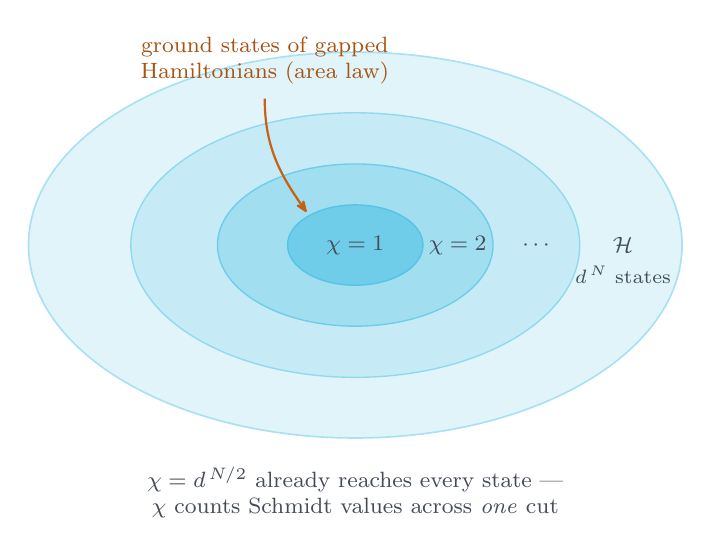
\begin{tikzpicture}[sub/.style={font=\footnotesize, color=ink!85},
                    >={Stealth[round,length=2.0mm]}]
  % nested MPS families: outermost is the whole Hilbert space
  \fill[tnbulk!18, draw=tnbulk!50, line width=0.6pt] (0,0) ellipse (4.15 and 2.45);
  \fill[tnbulk!34, draw=tnbulk!65, line width=0.5pt] (0,0) ellipse (2.85 and 1.68);
  \fill[tnbulk!56, draw=tnbulk!85, line width=0.5pt] (0,0) ellipse (1.75 and 1.03);
  \fill[tnbulk!85, draw=tnbulk,     line width=0.5pt] (0,0) ellipse (0.86 and 0.51);

  \node[sub] at (0,0)            {$\chi=1$};
  \node[sub] at (1.30,0)         {$\chi=2$};
  \node[sub] at (2.32,0)         {$\cdots$};
  \node[sub] at (3.40,0)         {$\mathcal H$};
  \node[sub, font=\scriptsize] at (3.40,-0.38) {$d^{\,N}$ states};
  \node[sub, anchor=north, align=center] at (0,-2.70)
    {$\chi=d^{\,N/2}$ already reaches every state ---\\
     $\chi$ counts Schmidt values across \emph{one} cut};

  % the corner physical states actually occupy
  \node[sub, color=tnbnd!85!black, anchor=south, align=center] at (-1.15,1.92)
    {ground states of gapped\\ Hamiltonians (area law)};
  \draw[->, tnbnd, line width=0.8pt] (-1.15,1.86) to[out=-90,in=125] (-0.62,0.42);
\end{tikzpicture}
\end{document}
